\begin{figure}[!h]
\centering
\resizebox{\textwidth}{!}{%
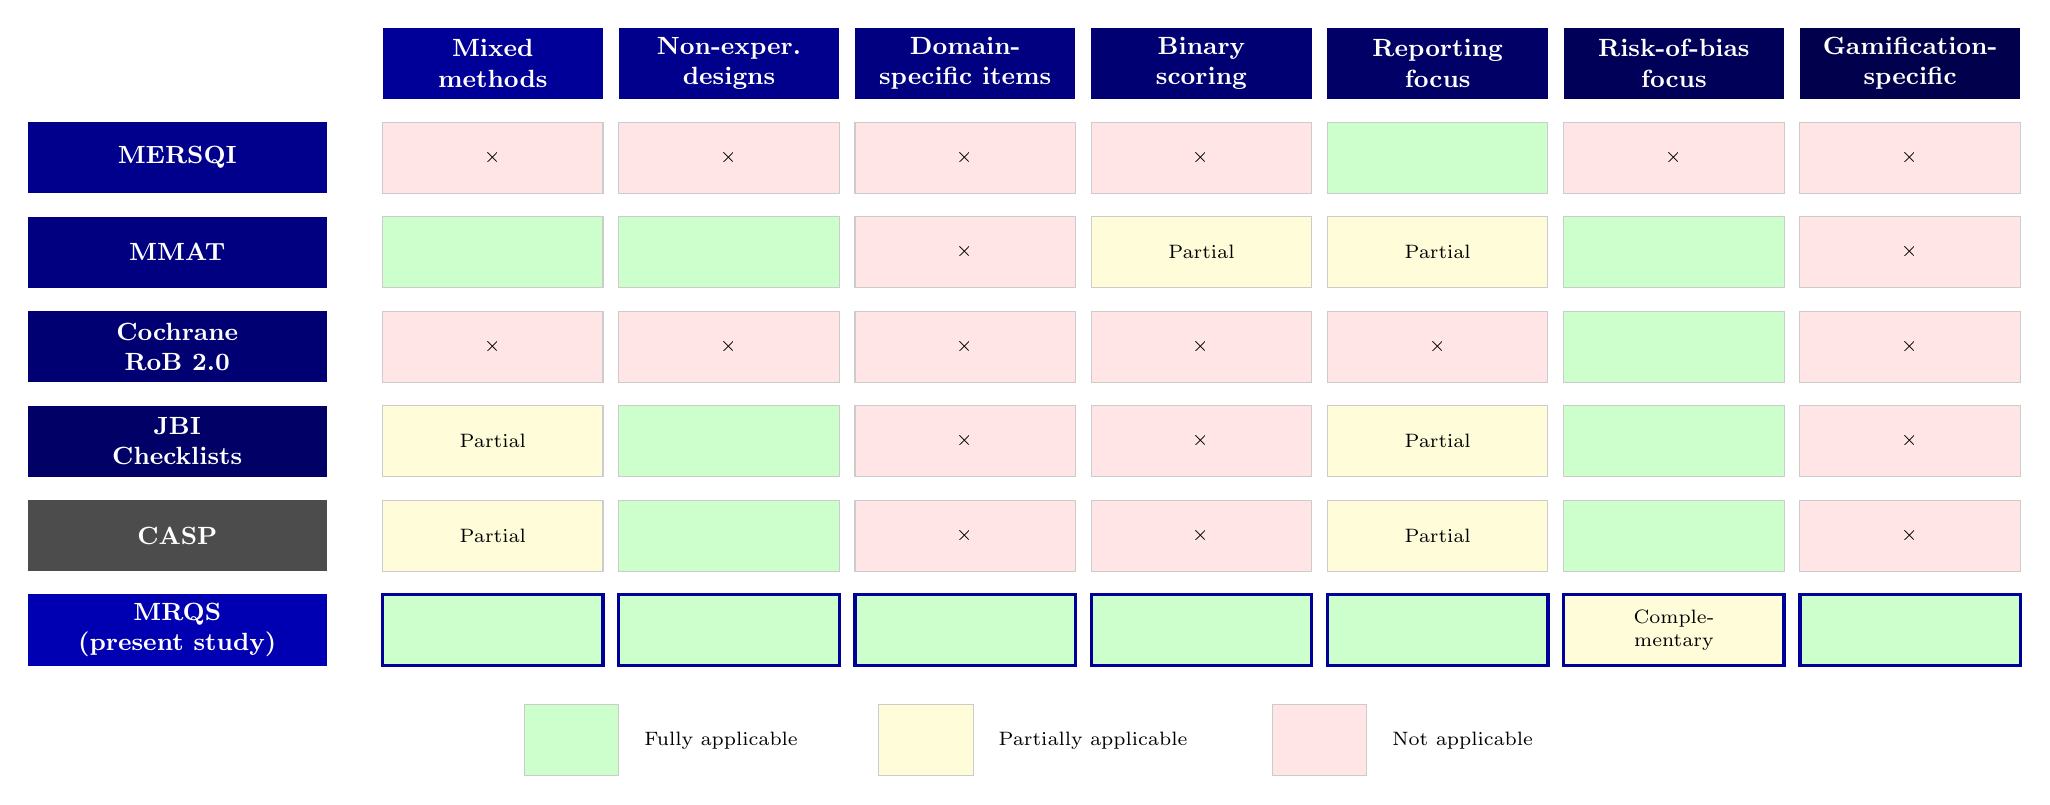
\begin{tikzpicture}[
  hdr/.style={font=\small\bfseries, text=white, minimum height=0.9cm,
    minimum width=2.8cm, align=center},
  rhdr/.style={font=\small\bfseries, text=white, minimum height=0.9cm,
    minimum width=3.8cm, align=center, anchor=east},
  cell/.style={rectangle, draw=gray!40, minimum height=0.9cm,
    minimum width=2.8cm, align=center, font=\scriptsize},
  strong/.style={cell, fill=green!20},
  moderate/.style={cell, fill=yellow!15},
  weak/.style={cell, fill=red!10},
  highlight/.style={cell, fill=green!20, draw=blue!60!black, line width=1.2pt},
  highlightr/.style={font=\small\bfseries, text=white, minimum height=0.9cm,
    minimum width=3.8cm, align=center, anchor=east, fill=blue!70!black},
]

% Column spacing
\def\colw{3.0}

% Column headers
\node[hdr, fill=blue!60!black] at (0, 0) {Mixed\\methods};
\node[hdr, fill=blue!55!black] at (\colw, 0) {Non-exper.\\designs};
\node[hdr, fill=blue!50!black] at (2*\colw, 0) {Domain-\\specific items};
\node[hdr, fill=blue!45!black] at (3*\colw, 0) {Binary\\scoring};
\node[hdr, fill=blue!40!black] at (4*\colw, 0) {Reporting\\focus};
\node[hdr, fill=blue!35!black] at (5*\colw, 0) {Risk-of-bias\\focus};
\node[hdr, fill=blue!30!black] at (6*\colw, 0) {Gamification-\\specific};

% Row 1: MERSQI
\node[rhdr, fill=blue!55!black] at (-2.1, -1.2) {MERSQI};
\node[weak] at (0, -1.2) {\texttimes};
\node[weak] at (\colw, -1.2) {\texttimes};
\node[weak] at (2*\colw, -1.2) {\texttimes};
\node[weak] at (3*\colw, -1.2) {\texttimes};
\node[strong] at (4*\colw, -1.2) {\checkmark};
\node[weak] at (5*\colw, -1.2) {\texttimes};
\node[weak] at (6*\colw, -1.2) {\texttimes};

% Row 2: MMAT
\node[rhdr, fill=blue!50!black] at (-2.1, -2.4) {MMAT};
\node[strong] at (0, -2.4) {\checkmark};
\node[strong] at (\colw, -2.4) {\checkmark};
\node[weak] at (2*\colw, -2.4) {\texttimes};
\node[moderate] at (3*\colw, -2.4) {Partial};
\node[moderate] at (4*\colw, -2.4) {Partial};
\node[strong] at (5*\colw, -2.4) {\checkmark};
\node[weak] at (6*\colw, -2.4) {\texttimes};

% Row 3: Cochrane RoB 2.0
\node[rhdr, fill=blue!45!black] at (-2.1, -3.6) {Cochrane\\RoB 2.0};
\node[weak] at (0, -3.6) {\texttimes};
\node[weak] at (\colw, -3.6) {\texttimes};
\node[weak] at (2*\colw, -3.6) {\texttimes};
\node[weak] at (3*\colw, -3.6) {\texttimes};
\node[weak] at (4*\colw, -3.6) {\texttimes};
\node[strong] at (5*\colw, -3.6) {\checkmark};
\node[weak] at (6*\colw, -3.6) {\texttimes};

% Row 4: JBI Checklists
\node[rhdr, fill=blue!40!black] at (-2.1, -4.8) {JBI\\Checklists};
\node[moderate] at (0, -4.8) {Partial};
\node[strong] at (\colw, -4.8) {\checkmark};
\node[weak] at (2*\colw, -4.8) {\texttimes};
\node[weak] at (3*\colw, -4.8) {\texttimes};
\node[moderate] at (4*\colw, -4.8) {Partial};
\node[strong] at (5*\colw, -4.8) {\checkmark};
\node[weak] at (6*\colw, -4.8) {\texttimes};

% Row 5: CASP
\node[rhdr, fill=gray!60!black] at (-2.1, -6.0) {CASP};
\node[moderate] at (0, -6.0) {Partial};
\node[strong] at (\colw, -6.0) {\checkmark};
\node[weak] at (2*\colw, -6.0) {\texttimes};
\node[weak] at (3*\colw, -6.0) {\texttimes};
\node[moderate] at (4*\colw, -6.0) {Partial};
\node[strong] at (5*\colw, -6.0) {\checkmark};
\node[weak] at (6*\colw, -6.0) {\texttimes};

% Row 6: MRQS (present study) — highlighted
\node[highlightr] at (-2.1, -7.2) {MRQS\\(present study)};
\node[highlight] at (0, -7.2) {\checkmark};
\node[highlight] at (\colw, -7.2) {\checkmark};
\node[highlight] at (2*\colw, -7.2) {\checkmark};
\node[highlight] at (3*\colw, -7.2) {\checkmark};
\node[highlight] at (4*\colw, -7.2) {\checkmark};
\node[moderate, draw=blue!60!black, line width=1.2pt] at (5*\colw, -7.2) {Comple-\\mentary};
\node[highlight] at (6*\colw, -7.2) {\checkmark};

% Legend
\node[strong, minimum width=1.2cm] at (1.0, -8.6) {};
\node[font=\scriptsize, anchor=west] at (1.8, -8.6) {Fully applicable};
\node[moderate, minimum width=1.2cm] at (5.5, -8.6) {};
\node[font=\scriptsize, anchor=west] at (6.3, -8.6) {Partially applicable};
\node[weak, minimum width=1.2cm] at (10.5, -8.6) {};
\node[font=\scriptsize, anchor=west] at (11.3, -8.6) {Not applicable};

\end{tikzpicture}%
}% end resizebox
\caption{Applicability of quality assessment tools to gamification research in history education. The MRQS (highlighted), developed for the present study, is the only instrument that simultaneously handles mixed-methods designs, includes domain-specific items, and uses binary scoring for reliability. Risk-of-bias assessment is addressed through a complementary adapted ROBIS instrument (see Section~\ref{sec:mrqs}).}
\label{fig:quality-tool-comparison}
\end{figure}
